\documentclass[utf-8]{beamer}
\usepackage{ctex}
\usetheme{CambridgeUS}
\setCJKsansfont{SimSun}
\setsansfont{Times New Roman}

\begin{document}
    \title{课前演讲}
    \subtitle{——《丰乳肥臀》莫言}
    \author{Garen}
    \date{\today}

    \titlepage
    \begin{frame}{目录}
        \tableofcontents
    \end{frame}

    \begin{section}{作者简介}
        \begin{frame}{作者简介}
            \begin{center}
                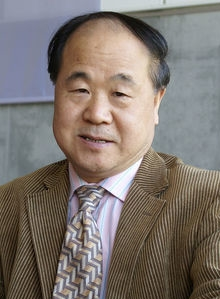
\includegraphics[width=100]{author_image.jpg}
            \end{center}
            \pause
            \begin{flushleft}
              \begin{itemize}
                \item 莫言,原名管谟业,1955年2月17日出生于山东高密,中国作家协会副主席、2012年诺贝尔文学奖获得者,亦是第一个获得诺贝尔文学奖的中国籍作家,获奖理由是:通过幻觉现实主义将民间故事、历史与当代社会融合在一起。作品深受魔幻现实主义影响。%可小谈“莫言”名字的来历
              \end{itemize}
            \end{flushleft}
        \end{frame}
    \end{section}

    \begin{section}{不要误解}
        \begin{frame}{不要误解}
            \begin{itemize}
            \item 看到这个标题,大家一般都会误解这本书的内容。
            \pause
            \item 而小说的正文开头就有这么一句话:
            \pause
            \item \textcolor[rgb]{1.00,0.00,0.00}{谨以此书献给母亲在天之灵}
            \pause
            \item 又试问:“丰乳”和“肥臀”寓意着什么?%生孩子好。也就代表母亲
            \pause
            \item 应该理解为:这是一本主要内容为\textbf{歌颂母亲}的小说。s
            \end{itemize}
        \end{frame}
    \end{section}
    \begin{section}{故事简介}
        \begin{frame}{故事简介}
            \pause
            \begin{itemize}
              \item 小说在抗日战争到改革开放的时间段内,以上官家唯一的男丁上官金童为第一视角,描述了上官家族间发生的种种故事。
              \pause
              \item 小说刻画了可歌可泣的母亲形象,集中体现了母爱的伟大无私,但通过上官金童的遭遇,也透露出一定的讽刺。
              \pause
              \item 小说细节十分的多,许多细节体现了作者的思想感情。
            \end{itemize}
        \end{frame}
    \end{section}

    \begin{section}{其他内容}
        \begin{frame}{家庭}
            \pause
            \begin{itemize}
              \item 上官金童共有七个姐姐,他是母亲唯一的儿子。
              \pause
              \item 他的七个姐姐的名字分别是:
              \pause
              \begin{itemize}
                \item 上官来弟
                \item 上官招弟
                \item 上官领弟
                \item 上官想弟
                \item 上官盼弟
                \item 上官念弟
                \item 上官求弟
              \end{itemize}
              \pause
              \item 母亲的那一胎是龙凤胎,儿女分别叫上官金童和上官玉女。
              \pause
              \item 在看到玉女的时候,母亲说了一句话:“\textbf{你呀,多余了}。”%你是多余的。
              \pause
              \item 他们的家庭命运多舛,可以说是战乱时期家庭的缩影。
            \end{itemize}
        \end{frame}
        \begin{frame}{上官金童}%贾宝玉式的人物
            \pause
            \begin{itemize}
              \item 上官金童是母亲与一个瑞典传教士的私生子。因此他有金色的头发。%为什么金童会是一个私生子?
              \pause
              \item 他名义上的父亲无法生育。并不是母亲的错。%并且金童的七个姐姐都是别人的种
              \pause
              \item 作为上官家唯一的儿子,他童年被几乎所有人优待。%在所谓“雪集”上,“我”扮演雪公子,母亲、姐姐们的偏爱
              \pause
              \item 母亲对儿子抱有很大的期望,也对儿子有强烈的爱,可惜儿子没让母亲满意过。%母亲意味深长的一句话。
              \pause
              \item 青年时期正是文革,因罪被判刑十五年。直接失去人生的黄金时光。
              \pause
              \item 他没有主见,没有男子气概,事情总是任人摆布,而恋乳癖的疾病更是加剧了这一特点。%最霸道的事情、最威风的事情。哭
              \pause
              \item 上官金童一生\textbf{懦弱无能},最终成为了\textbf{一无所有}的人。%最终被妻子夺取了仅存的一切
              \pause
              \item 上官金童是中国近代知识分子、近代社会的一种缩影。%我毫不避讳地承认:上官金童是我的精神写照。
            \end{itemize}
        \end{frame}
        \begin{frame}{母亲}
            \pause
            \begin{itemize}
                \item 母亲名为上官鲁氏,从5岁裹脚到16岁。后嫁进了打铁的上官家。
                \pause
                \item 母亲因为迟迟生不出儿子,遭到上官家\textcolor[rgb]{1.00,0.00,0.00}{极}不公平的待遇。%生七姐后、生金童之前还跑去给驴接生
                \pause
                \item 家庭支离破碎,母亲肩负起支撑起家庭的重担,养活了所有的儿女以及外孙女,\textbf{没有抛弃过任何的儿女。}
                \pause
                \item 伟大的母亲抚养了这些儿女,可儿女们有的却让母亲失望(尤其是上官金童)。
                \pause
                \item 寿九五而终,她最后被上官金童埋在沼泽地里头。
                \pause
                \item 母亲受了一生的苦难,是近代中国母亲的影子。母亲是崇高的,是伟大的。
                \pause
                \item 莫言在《丰乳肥臀》出版后,曾说:“为什么会有崇高?——苦难。苦难使人崇高。母亲几乎忍受了所有苦难:战争、饥饿、贫穷、疾病;在层出不穷的苦难中,母亲变得崇高了。”
            \end{itemize}
        \end{frame}
    \end{section}

    \begin{frame}{故事背景}
        \begin{itemize}
          \pause
          \item 小说发生的背景之一是抗日战争时期。饥饿、贫穷、困苦的生活始终围绕着那个年代的人。%母亲生金童的时候,外面就出了天大的事故。
          \pause
          \item 生活在高密乡,家乡的风俗、思想习惯贯穿于小说之中。
          \pause
          \item 许多人的去向与故事情节的发展有关。
        \end{itemize}
    \end{frame}
    \begin{frame}{艺术手法}
        \begin{itemize}
            \pause
            \item 莫言的比喻句、心理描写特别秀,细节十分精彩。%不念给你们听。不然就没了。
            \pause
            \item 民间故事、魔幻现实主义等的融合,是莫言小说的精彩之处。
            \pause
            \item e.g. 上官金童的三姐上官领弟在精神错乱后成为了“鸟仙”!
            \pause
            \item 夸张的描写,更是加强了小说的讽刺力度。
            \pause
            \item e.g. 在打日本鬼子的时候,村民们就用了“屎尿战”来对付他们。
            \pause
            \item e.g. 主人公上官金童的恋乳癖是他懦弱无能的诱因和夸张体现。
        \end{itemize}
    \end{frame}
    \begin{frame}{其他}
        \pause
        \begin{itemize}
            \item 这本书一开始出版的时候,被人认为是反动小说。%不是因为题目,而是因为不招共产党喜欢
            \pause
            \item 不过在文学里扯政治,就不在我想讲的范畴。
            \pause
            \item “2013年,导演张艺谋称要将作品《丰乳肥臀》搬上银幕。” ???%无影无迹
        \end{itemize}
    \end{frame}
    \begin{section}{结尾}
        \begin{frame}
            \pause
            \begin{itemize}
              \item 这本书那么长,当然不会建议大家现在去读的。
              \pause
              \item 但是莫言的书,值得一读!
            \end{itemize}
            \pause
            \begin{center}\huge
                谢谢!
            \end{center}
            \pause
            \begin{flushright}
                all made by \LaTeX
            \end{flushright}
        \end{frame}
    \end{section}
\end{document} 